\documentclass[11pt]{article}
\ifdefined\pdfgentounicode
\pdfgentounicode=1
\input{glyphtounicode-cmex}
\fi
\usepackage[T1]{fontenc}
\usepackage{lmodern}
\usepackage[margin=1.05in]{geometry}
\usepackage{amsmath,amssymb,amsthm,mathtools}
\usepackage{microtype}
\usepackage{xcolor}
\usepackage{tikz}
\usepackage{hyperref}
\hypersetup{colorlinks=true,linkcolor=blue!45!black,citecolor=blue!45!black,
 urlcolor=blue!45!black,pdftitle={Subpolynomial dimension reduction in Lp},
 pdfauthor={OpenAI}}
\usepackage{bookmark}

\newcommand{\R}{\mathbb R}
\newcommand{\E}{\mathbb E}
\newcommand{\Prob}{\mathbb P}
\newtheorem{theorem}{Theorem}[section]
\newtheorem{lemma}[theorem]{Lemma}
\newtheorem{proposition}[theorem]{Proposition}
\theoremstyle{remark}
\newtheorem{remark}[theorem]{Remark}
\numberwithin{equation}{section}
\setlength{\emergencystretch}{1em}
\setlength{\parskip}{0.2em}
\widowpenalty=10000
\clubpenalty=10000

\title{Subpolynomial dimension reduction in $L_p$}
\author{OpenAI}
\date{September 23, 2026}

\begin{document}
\maketitle
\begin{abstract}
For every fixed $1<p<\infty$ and $D>1$, every $n$-point subset of a
real $L_p$ space embeds into $\ell_p^d$ with distortion at most $D$
and subpolynomial dimension $d=n^{o(1)}$. The target has the same
exponent $p$, and the embedding need not be linear.
\end{abstract}

\section{Introduction}

The Johnson--Lindenstrauss lemma places every $n$-point subset of a
Hilbert space in $O_D(\log n)$ Euclidean dimensions with any prescribed
distortion $D>1$~\cite[Lemma~1]{JohnsonLindenstrauss1984}.
Johnson and Lindenstrauss also asked what analogues of their lemma hold
in other Banach spaces~\cite[Problem~3]{JohnsonLindenstrauss1984}.
For other $L_p$ spaces, the corresponding finite-metric question must
be distinguished both from discretizing an entire linear subspace and
from requiring the embedding itself to be linear. We study the
coordinate-target version: the points may be repositioned freely, but
their images must lie in $\ell_p^d$ with the same exponent $p$.
For the broader dimension-reduction landscape and the distinction
between coordinate targets and arbitrary subspaces, see
Naor~\cite{Naor2018}.

All spaces and maps in this paper are real. For $1<p<\infty$, an integer
$n\ge2$, and $D\ge1$, let $d_p(n,D)$ be the least integer $d$ such that
every $n$-point subset $\{x_1,\ldots,x_n\}$ of any $L_p$ space admits
images $y_1,\ldots,y_n\in\ell_p^d$ and a number $s>0$ satisfying
\begin{equation}\label{eq:distortion}
 s\|x_i-x_j\|_p\le \|y_i-y_j\|_p
 \le Ds\|x_i-x_j\|_p\qquad(i,j\in\{1,\ldots,n\}).
\end{equation}
The maps are unrestricted; in particular, they need not extend linearly
to the ambient space. Lemma~\ref{lem:exact-upper} below shows that the
same quantity results if the input sets are restricted to finite
coordinate spaces $\ell_p^m$.

\begin{theorem}\label{thm:main}
Fix $1<p<\infty$, $p\ne2$, and put
\[
 \gamma(p)=
 \begin{cases}
  2-p,&1<p<2,\\
  1-2/p,&2<p<\infty.
 \end{cases}
\]
For every $D>1$ there is a constant $C_{p,D}<\infty$ such that, for
every integer $n\ge2$,
\begin{equation}\label{eq:main-bounds}
 \frac{\log n}{\log(1+2D)}
 \le d_p(n,D)
 \le \exp\!\bigl(C_{p,D}(\log n)^{\gamma(p)}\bigr).
\end{equation}
For exact embeddings,
\begin{equation}\label{eq:exact-bounds}
 \left\lfloor\frac{n-1}{4}\right\rfloor^2
 \le d_p(n,1)\le\binom n2\qquad(n\ge9).
\end{equation}
Consequently,
\[
 \lim_{n\to\infty}\frac{\log d_p(n,D)}{\log n}
 =\begin{cases}0,&D>1,\\2,&D=1.\end{cases}
\]
\end{theorem}

The constants in the upper bound depend on the fixed parameters $p,D$;
no uniformity as $p$ approaches an endpoint or $D$ approaches $1$ is
asserted. For $p=2$, the classical Hilbert result gives the stronger
bound $d_2(n,D)=O_D(\log n)$ for every fixed $D>1$.
The theorem is existential and does not assert an efficient embedding
algorithm.

\subsection{Earlier results and the exact-distortion contrast}

Ball proved the exact-coordinate upper bound $\binom n2$ and its
quadratic-order sharpness for $1\le p<2$~\cite{Ball1990}.
Lemma~\ref{lem:exact-upper} recalls the distance-cone and
Carath\'eodory argument for that upper bound. The lower bound in
\eqref{eq:exact-bounds} uses an antipodal row-and-column configuration.
Its disjoint-support test is the classical equality criterion for the
$p$-parallelogram defect~\cite[Corollary~2.1]{Lamperti1958}; in particular,
the argument includes even integers $p>2$.

Approximate finite-set bounds and linear-subspace discretization have
different dimension parameters. Below $2$, Schechtman's finite-set
estimates progressed from $O_D(n\log n)$ coordinates to
$O_{p,D}(n)$~\cite{Schechtman1987,Schechtman2011}.
The subspace results of Bourgain--Lindenstrauss--Milman and Talagrand
instead preserve all vectors in a given $r$-dimensional subspace by a
linear map~\cite{BourgainLindenstraussMilman1989,Talagrand1995}.
Applying such a theorem to the span of the translated data gives
$r\le n-1$;
it does not give the present subpolynomial bound in cardinality.
Bourgain's embedding of arbitrary finite metrics into Hilbert space
allows distortion growing with $n$~\cite{Bourgain1985}, another
different guarantee.

The absence of a linearity requirement is essential: fixed-distortion
linear maps on selected $L_p$ configurations can require dimension
proportional to their cardinality when $p\ne2$
\cite[Section~3]{LeeMendelNaor2005}.
At the endpoint $p=1$, the obstruction of Brinkman--Charikar applies
even to nonlinear maps; see also Lee--Naor's proof
\cite{BrinkmanCharikar2005,LeeNaor2004}.
For $p>2$, Naor--Ren's recent lower bound
\cite[Section~1.1, equation~(2)]{NaorRen2026Threshold} rules out
$O_{p,D}(\log n)$ coordinate dimension: along arbitrarily large
cardinalities it requires dimension of order at least
$(\log n/(\log\log n)^2)^{p/2}$ at fixed distortion.
This is compatible with \eqref{eq:main-bounds}; neither its upper
exponent nor its elementary logarithmic lower bound is asserted to be
optimal.

The dependence on cardinality also distinguishes this problem from embedding
one infinite space into a fixed finite-dimensional target. A metric space is
\emph{doubling} if every ball can be covered by a fixed number of balls of
half its radius. A separate construction gives an infinite doubling subset
of real Hilbert space with no bi-Lipschitz embedding into any
finite-dimensional Euclidean space at any finite distortion
\cite{OpenAI2026DoublingHilbert}. This is compatible with finite-set
dimension reduction and is not an input to our proof.

\subsection{Method and organization}

Our starting point is a bounded distribution of scalar images of the
input points. After dividing each increment by the corresponding
original distance, we seek nearly equal $p$th moments for every pair.
Lemma~\ref{lem:weighted} reduces this simultaneous requirement to a
weighted-average condition for each strictly positive probability on
the pairs. Crucially, the common moment $b$ and magnitude bound $K$
are uniform over those probabilities. Convex separation produces one
distribution working for all pairs; independent sampling then supplies
the coordinates of a finite embedding.
This sampling step belongs to Maurey's empirical method, as presented
by Pisier~\cite{Pisier1981}. A close distance-matrix antecedent
is Eskenazis's use of that method for incompressible sets
\cite[Sections~1.3 and~2.1]{Eskenazis2024}; that theorem controls
additive errors, with a bound depending on the incompressibility of
the data. Here the weighted-moment construction supplies the uniform
relative control needed for arbitrary configurations.

The geometric input in Section~\ref{sec:projection} is a projection
onto normalized increments that come from scalar labels on the
points. It is an $L_2$ contraction for a suitable choice of pair
weights, and its $L_\infty$ norm is $O(\log n)$.
We obtain the latter property by a fixed-point reweighting of the
electrical-flow localization estimate of Gurel-Gurevich, Nachmias,
and Sachdeva~\cite[Theorem~1.3]{GGNS}.
Their estimate improves the earlier $O(\log^2 n)$ localization bound
of Schild--Rao--Srivastava~\cite[Theorem~1.5, preprint version]{SRS18}.
Appendix~\ref{app:localization} presents the heat-kernel and entropy
proof from~\cite[Sections~2--4]{GGNS} in our notation.

After the common homogeneous-increment and signed-Poisson setup,
the two ranges require different random increments.
Section~\ref{sec:below} constructs symmetric $p$-stable marginals,
clips them, and projects back to consistent increments.
Stable projections and truncated heavy-tail moments have earlier
geometric uses, including Indyk's work~\cite{Indyk06};
the required marginal construction and tail bounds are proved here.
For $p>2$, Section~\ref{sec:above} uses overlapping magnitude
truncations followed by signed Poisson sampling. Their overlap
enlarges the input energy relative to the projection error.
The moment comparison is of Rosenthal type
\cite{Rosenthal70,Pinelis15}; Appendix~\ref{app:poisson} proves the
specific leading coefficient $1+\epsilon$ needed for distortion
arbitrarily close to one. The final main-text section inserts the resulting
$b,K$ into the sampling estimate and proves the packing and exact
embedding lower bounds.

We use finite-dimensional convexity, Brouwer's fixed-point theorem,
and standard probability; the specialized electrical-localization and
Poisson-moment arguments are supplied in the appendices.

Throughout, logarithms are natural. Constants $C,c>0$ are absolute;
subscripts indicate the parameters on which a constant may depend.
Their values may change from line to line.

\section{Finite coordinates and normalized increments}

\begin{lemma}[Exact discretization]\label{lem:exact-upper}
Every $n$-point subset of a real $L_p$ space embeds isometrically into
$\ell_p^{\binom n2}$. This holds for every $1\le p<\infty$.
\end{lemma}

\begin{proof}
Let the points be $x_1,\ldots,x_n\in L_p(\mu)$, and let $E$ be the set
of unordered pairs of distinct indices. Write $N=|E|$. Choose measurable
representatives, finite outside a common null set, and put
\[
 q(t)=\bigl(|x_i(t)-x_j(t)|^p\bigr)_{ij\in E},\qquad
 s(t)=\sum_{e\in E}q_e(t),\qquad S=\int s\,d\mu.
\]
The points are distinct, so $0<S<\infty$. Consider the compact set
\[
 \mathcal K=\left\{
  \bigl(|z_i-z_j|^p\bigr)_{ij\in E}:
  z\in\R^n,\ z_n=0,\ \sum_{ij\in E}|z_i-z_j|^p=1
 \right\}\subset\R^E.
\]
Compactness follows because its defining set of labels is closed and
$|z_i|\le1$ for every $i$. For $s(t)>0$, the vector $q(t)/s(t)$ belongs
to $\mathcal K$. Hence
\[
 \frac1S\int q(t)\,d\mu(t)
 =\int_{\{s>0\}}\frac{q(t)}{s(t)}\,\frac{s(t)}S\,d\mu(t)
 \in\operatorname{conv}(\mathcal K).
\]
Here a barycenter belongs to the convex hull because that convex hull
is compact; equivalently, this follows by finite-dimensional separation
\cite[Theorems~11.3 and~17.2]{Rockafellar1970}.
The set $\mathcal K$ lies in the affine hyperplane whose coordinates
sum to one. By Carath\'eodory's theorem
\cite[Theorem~17.1]{Rockafellar1970}, the displayed vector is a
convex combination of at most $N$ points of $\mathcal K$. Choose
corresponding labels $z^{(a)}$ and coefficients $\theta_a\ge0$ with
$\sum_a\theta_a=1$. Then
\[
 y_i=\bigl((S\theta_a)^{1/p}z_i^{(a)}\bigr)_a
\]
satisfies $\|y_i-y_j\|_p^p=\|x_i-x_j\|_p^p$ for every pair.
\end{proof}

For the upper bound in~\eqref{eq:main-bounds}, we may therefore fix
distinct points $x_1,\ldots,x_n\in\ell_p^m$ for some finite $m$.
Give the complete graph on $\{1,\ldots,n\}$ an arbitrary orientation,
and use $e=ij$ to denote an edge with this ordering. Set
\[
 \delta_e=\|x_i-x_j\|_p>0,\qquad
 V=\left\{\left(\frac{z_i-z_j}{\delta_e}\right)_{e=ij\in E}:
 z\in\R^n\right\}\subset\R^E.
\]
We call elements of $V$ \emph{normalized gradients}. Each such vector
determines scalar labels $z_i$ uniquely after imposing $z_n=0$; this
choice is linear in the vector. Thus a collection of normalized
gradients can always be used as the coordinates of one map on the
given points.

For a strictly positive probability vector $\sigma=(\sigma_e)_{e\in E}$,
write
\[
 \|f\|_{2,\sigma}^2=\sum_{e\in E}\sigma_e|f_e|^2.
\]
We first state the moment criterion that our random gradients must satisfy.

\section{From weighted moments to an embedding}

A random normalized gradient gives candidate scalar coordinates. We seek
one bounded distribution whose $p$th moments are nearly equal on every
edge. The next lemma shows that it is enough to meet each weighted test
separately, even though the distribution may change with the test
probability. The common moment and magnitude bound must remain fixed.

The common moment $b$ below is allowed to grow: multiplying all
distances by the same factor does not change distortion. This freedom
will let us absorb an additive error in the moment estimates.

\begin{lemma}[Weighted moment criterion]\label{lem:weighted}
Let $0<\eta<1/3$ and $b,K\ge1$. Suppose that, for every strictly
positive probability vector $\lambda$ on $E$, there is a random
normalized gradient $F\in V$ such that
\begin{equation}\label{eq:weighted-target}
 \|F\|_\infty\le K\quad\text{almost surely},\qquad
 \sum_{e\in E}\lambda_e\left|\E|F_e|^p-b\right|\le\eta b.
\end{equation}
The numbers $b$ and $K$ are the same for all $\lambda$. Then the points
admit an embedding into $\ell_p^d$ with distortion at most
\[
 \left(\frac{1+3\eta}{1-3\eta}\right)^{1/p},
\]
where
\begin{equation}\label{eq:sampling-dimension}
 d\le\left\lceil
 C\max\left\{1,\frac{K^{2p}}{\eta^2b^2}\right\}\log(2n)
 \right\rceil
\end{equation}
for an absolute constant $C$.
\end{lemma}

\begin{proof}
Let $\mathcal C$ be the convex hull of the compact set
\[
 \left\{\bigl(|f_e|^p\bigr)_{e\in E}: f\in V,\ \|f\|_\infty\le K\right\}.
\]
It is compact and consists exactly of the moment vectors of
distributions of such gradients; finite mixtures suffice by
Carath\'eodory's theorem. We claim that $\mathcal C$ meets the open box
\[
 \mathcal B=\{m\in\R^E: |m_e-b|<2\eta b\text{ for all }e\}.
\]
Otherwise, finite-dimensional separation
\cite[Theorem~11.3]{Rockafellar1970} gives a vector $a\ne0$ such that, after
normalizing $\sum_e|a_e|=1$,
\[
 \sum_e a_e(m_e-b)\ge2\eta b\qquad(m\in\mathcal C).
\]
Apply the hypothesis with
$\lambda_e=\frac34|a_e|+\frac1{4|E|}$. Its moment vector $m\in\mathcal C$
satisfies
\[
 \sum_e a_e(m_e-b)
 \le\sum_e|a_e||m_e-b|
 \le\frac43\sum_e\lambda_e|m_e-b|
 \le\frac43\eta b,
\]
a contradiction. Thus there is one distribution of gradients,
still bounded by $K$, for which every expected $p$th moment differs
from $b$ by less than $2\eta b$.

For completeness, we prove a Hoeffding-type bounded-sum estimate for the
sampling step, with constants weaker than the classical bound in
\cite[Theorem~2, p.~16, equation~(2.6)]{Hoeffding1963}.
If $0\le X\le K^p$ and $X'$ is an independent copy, Jensen's
inequality and symmetry give
\[
 \E e^{t(X-\E X)}
 \le\E e^{t(X-X')}
 =\E\cosh\bigl(t(X-X')\bigr)
 \le e^{t^2K^{2p}/2},
\]
using $\cosh u\le e^{u^2/2}$. Take $d$ independent samples
$F^{(1)},\ldots,F^{(d)}$ from the preceding distribution. Apply this
bound to $X=|F_e|^p$, multiply moment generating functions, and use
Markov's inequality with $t=\eta b/K^{2p}$. Applying the same argument
to the lower tail gives
\[
 \Prob\left(
 \left|\frac1d\sum_{a=1}^d|F_e^{(a)}|^p-\E|F_e|^p\right|>\eta b
 \right)
 \le2\exp\left(-\frac{d\eta^2b^2}{2K^{2p}}\right).
\]
For the value in~\eqref{eq:sampling-dimension} with $C$ sufficiently
large, a union bound over $|E|<n^2/2$ edges is less than one. Choose
an outcome for which all empirical moments belong to
$[(1-3\eta)b,(1+3\eta)b]$. Realize each $F^{(a)}$ by scalar labels
$z_i^{(a)}$, and set
\[
 y_i=d^{-1/p}\bigl(z_i^{(1)},\ldots,z_i^{(d)}\bigr).
\]
Then
\[
 \frac{\|y_i-y_j\|_p^p}{\delta_{ij}^p}
 =\frac1d\sum_{a=1}^d|F_{ij}^{(a)}|^p.
\]
This proves the assertion, with scale $s=((1-3\eta)b)^{1/p}$.
\end{proof}

\section{A projection with controlled row sums}
\label{sec:projection}

The projection estimate follows from the electrical-flow localization theorem
of Gurel-Gurevich, Nachmias, and Sachdeva~\cite[Theorem~1.3]{GGNS}.
For a matrix $T$, write $|T|$ for its entrywise absolute value.

\begin{lemma}[Electrical-flow localization]\label{lem:localization}
Let $G$ be a connected loopless graph on $n\ge2$ vertices, let $B$ be an oriented
edge-by-vertex incidence matrix, and let $C=\operatorname{diag}(c_e)$ with
$c_e>0$. If $Q$ is the Euclidean orthogonal projection onto
$\operatorname{im}(C^{1/2}B)$, then
\begin{equation}\label{eq:localization}
  \bigl\|\,|Q|\,\bigr\|_{2\to2}\le 2\log n.
\end{equation}
\end{lemma}

The proof is given in Appendix~\ref{app:localization}.


We now apply this estimate to the normalized-gradient space $V$. Set
\begin{equation}\label{eq:H}
 H=4\log(2n).
\end{equation}

\begin{lemma}[Weighted projection]\label{lem:projection}
For every strictly positive probability vector $\lambda$ on $E$, there
is a probability vector $\sigma$ with $\sigma_e\ge\lambda_e/2$ such
that the orthogonal projection $P$ onto $V$ in $\ell_2(\sigma)$ satisfies
\begin{equation}\label{eq:projection-row-sums}
 \max_{e\in E}\sum_{f\in E}|P_{ef}|\le H.
\end{equation}
In particular, $\|P\|_{\infty\to\infty}\le H$, and both $P$ and
$I-P$ are contractions on $\ell_2(\sigma)$.
\end{lemma}

\begin{proof}
Let $B$ be the incidence matrix of the oriented complete graph fixed above.
For a strictly positive probability vector $\sigma$, denote the weighted
orthogonal projection by $P(\sigma)$, and put
\[
 D_\sigma=\operatorname{diag}(\sqrt{\sigma_e}),\qquad
 C_\sigma=\operatorname{diag}(\sigma_e/\delta_e^2).
\]
Then $Q(\sigma)=D_\sigma P(\sigma)D_\sigma^{-1}$ is the Euclidean
orthogonal projection onto $\operatorname{im}(C_\sigma^{1/2}B)$.
Define $R_e(\sigma)=\sum_f|P(\sigma)_{ef}|$. Since
$\|\sqrt\sigma\|_2=1$, Lemma~\ref{lem:localization} gives
\begin{equation}\label{eq:average-row-sums}
 \sum_e\sigma_e R_e(\sigma)^2
   =\bigl\|\,|Q(\sigma)|\sqrt\sigma\,\bigr\|_2^2
   \le (2\log n)^2.
\end{equation}

To control every row, we choose weights that allocate more mass to
rows with large absolute sums. Consider the compact convex set
\[
 \Sigma=\left\{\sigma:\ \sum_e\sigma_e=1,
                         \ \sigma_e\ge\lambda_e/2\right\}.
\]
The weighted projection, and hence every $R_e$, depends continuously on
$\sigma\in\Sigma$: in a fixed basis of $V$, its formula involves the
inverse of a positive definite Gram matrix. Set
\[
 u_e(\sigma)=\frac{\sigma_eR_e(\sigma)^2}{2(2\log n)^2},
 \qquad
 \Phi_e(\sigma)=u_e(\sigma)
       +\left(1-\sum_f u_f(\sigma)\right)\lambda_e.
\]
By \eqref{eq:average-row-sums}, $\sum_eu_e(\sigma)\le1/2$.
Thus $\Phi$ is a continuous self-map of $\Sigma$, and Brouwer's theorem
\cite[Corollary~2.15]{Hatcher2002} provides a fixed point.
At that fixed point $u_e(\sigma)\le\sigma_e$;
since $\sigma_e>0$, this gives
\[
 R_e(\sigma)\le2\sqrt2\log n\le H.
\]
The remaining assertions follow from the row-sum formula for the
$\ell_\infty$ operator norm and orthogonality in $\ell_2(\sigma)$.
\end{proof}

For the rest of the upper-bound argument, fix $D>1$ and choose
$0<\eta<1/6$ so that
\begin{equation}\label{eq:eta-choice}
 \left(\frac{1+3\eta}{1-3\eta}\right)^{1/p}\le D.
\end{equation}
For each strictly positive test probability $\lambda$, we will use
$\sigma$ and $P$ from Lemma~\ref{lem:projection}. It suffices to
construct $F$ with weighted error at most $\eta b/2$ under $\sigma$,
since $\lambda\le2\sigma$ coordinatewise. The parameters $b$ and $K$
will depend only on $p,\eta,n$.

\section{Homogeneous increments and signed Poisson sampling}

The following measure gives every normalized increment the same
magnitude distribution. On
$\Omega=(0,\infty)\times\{1,\ldots,m\}$, set
\[
 d\nu(r,t)=p r^{-p-1}\,dr
 \quad\text{on each copy indexed by }t,
 \qquad
 g_e(t)=\frac{x_i(t)-x_j(t)}{\delta_e},\qquad v_e(r,t)=r g_e(t).
\]
For every $(r,t)$, the vector $v(r,t)$ belongs to $V$. Since
$\sum_{t=1}^m|g_e(t)|^p=1$, direct integration gives
\begin{equation}\label{eq:powerlaw}
 \nu(|v_e|>a)=a^{-p}\qquad(a>0).
\end{equation}
More generally, for every nonnegative measurable function
$\phi:(0,\infty)\to[0,\infty]$,
\begin{equation}\label{eq:magnitude-density}
 \int_{\{v_e\ne0\}}\phi(|v_e|)\,d\nu
 =p\int_0^\infty\phi(u)u^{-p-1}\,du.
\end{equation}
In particular, $\nu(\max_e|v_e|>a)\le|E|a^{-p}$. The measure $\nu$
is not a probability measure. The second moment of the small jumps
is finite precisely when $p<2$; for $p>2$, the useful finite second
moment is instead in the large jumps. This leads to two different
uses of the same homogeneous increments.

We record the elementary sampling facts used in both ranges. On a
measurable region of finite mass $M$, \emph{signed Poisson sampling}
of a vector function $h$ means
\[
 W=\sum_{j=1}^{N}\varepsilon_j h(\omega_j),
\]
where $N$ has Poisson law of mean $M$, the $\omega_j$ are independent
with law $\nu/M$ restricted to the region, and the $\varepsilon_j$
are independent uniform signs. All these choices are independent.
For $M=0$ the sum is zero. Sampling on disjoint regions is independent:
indeed, subdividing a Poisson number of independent samples gives
independent Poisson counts, as is seen from their joint probability
generating function. In particular, sampling a $V$-valued function
produces a vector in $V$.

\begin{lemma}[Signed Poisson formulas]\label{lem:poisson}
Let $h$ be a bounded real function supported on a region of finite
$\nu$-measure, and let $S$ be its signed Poisson sum. Then
\begin{align}
 \E e^{itS}
 &=\exp\left(\int(\cos(th)-1)\,d\nu\right),\label{eq:poisson-cf}\\
 \E e^{tS}
 &=\exp\left(\int(\cosh(th)-1)\,d\nu\right),\label{eq:poisson-mgf}\\
 \E S&=0,\qquad \E S^2=\int h^2\,d\nu.\label{eq:poisson-variance}
\end{align}
The characteristic-function identity also holds for unbounded $h$
on a finite-measure region.
\end{lemma}

\begin{proof}
Conditioning on the Poisson count proves the first two formulas:
the expectation for one signed sample is respectively the average
of $\cos(th)$ or $\cosh(th)$, and the Poisson generating function is
$\E z^N=\exp(M(z-1))$. The variance formula follows by conditioning
as well.
\end{proof}

\section{The range \texorpdfstring{$1<p<2$}{1 < p < 2}}\label{sec:below}

Fix $1<p<2$. We construct the random normalized gradient required by
Lemma~\ref{lem:weighted}, with $\eta$ as chosen in~\eqref{eq:eta-choice}.

\subsection{A common heavy-tailed marginal}

We first construct a random vector $Y\in V$ by symmetric Poisson sampling
of the vector $v$ against the intensity $\nu$. On the region
$\{\|v\|_\infty>1\}$, this is an ordinary signed compound Poisson sum:
the region has measure at most $|E|$ by~\eqref{eq:powerlaw}. For each
$j\ge0$, independently sample the region
\[
 A_j=\{2^{-j-1}<\|v\|_\infty\le2^{-j}\},
\]
and denote its signed compound Poisson sum by $Y^{(j)}$.
Each $A_j$ has finite measure, at most $|E|2^{p(j+1)}$.
These are centered independent vectors. For every edge $e$,
\[
 \sum_{j\ge0}\E|Y^{(j)}_e|^2
 =\int_{0<\|v\|_\infty\le1}|v_e|^2\,d\nu
 \le\int_{0<|v_e|\le1}|v_e|^2\,d\nu
 =\frac{p}{2-p}.
\]
Consequently $\sum_{j\ge0}Y^{(j)}$ converges in $L_2$ with values in the
finite dimensional space $\R^E$. Adding the sum on
$\{\|v\|_\infty>1\}$ defines $Y$. Every partial sum belongs to $V$;
since $V$ is closed, $Y\in V$ almost surely.

The compound Poisson formula and convergence in probability give
\begin{equation}\label{eq:below-characteristic}
 \E e^{i\theta Y_e}
 =\exp\left(\int\bigl(\cos(\theta v_e)-1\bigr)\,d\nu\right)
 =\exp\left(p\int_0^\infty
       \bigl(\cos(\theta u)-1\bigr)u^{-p-1}\,du\right).
\end{equation}
The integrals converge absolutely: near zero the integrand is
$O_\theta(u^{1-p})$, and at infinity it is $O(u^{-p-1})$.
The second equality follows from~\eqref{eq:magnitude-density} and the evenness
of cosine. In particular, uniqueness of characteristic functions
\cite[Theorem~3.3.11]{Durrett2019} shows that all the $Y_e$ have the
same distribution, depending only on $p$.

For later use we prove directly that
\begin{equation}\label{eq:below-tail}
 c_p a^{-p}\le\Prob(|Y_e|>a)\le C_p a^{-p}
 \qquad(a\ge1).
\end{equation}
Fix $e$ and $a\ge1$. By Poisson splitting, or by the characteristic
function~\eqref{eq:below-characteristic}, $Y_e$ has the distribution
of an independent sum $B_a+S_a$. Here $B_a$ is the signed compound
Poisson sum on $\{|v_e|>a\}$, whose number $N_a$ of jumps is Poisson
with mean $a^{-p}$, while $S_a$ is the $L_2$ limit of the small-jump
sums on $\{0<|v_e|\le a\}$. Thus
\[
 \E S_a=0,
 \qquad
 \E|S_a|^2=\int_{0<|v_e|\le a}|v_e|^2\,d\nu
 =\frac{p}{2-p}a^{2-p}.
\]
Chebyshev's inequality gives
\[
 \Prob(|Y_e|>a)
 \le\Prob(N_a\ge1)+\Prob(|S_a|>a)
 \le\left(1+\frac{p}{2-p}\right)a^{-p}.
\]
For the reverse inequality, condition on $N_a=1$, the magnitude $u>a$
of its jump, and $S_a=s$. At least one of $|s+u|$ and $|s-u|$ exceeds
$a$, and the jump's two signs are equally likely. Therefore
\[
 \Prob(|Y_e|>a)
 \ge\frac12\Prob(N_a=1)
 =\frac12 a^{-p}e^{-a^{-p}}
 \ge\frac{1}{2e}a^{-p}.
\]
This proves~\eqref{eq:below-tail}.

\subsection{Clipping and projection}

Let $\lambda$ be a strictly positive probability on $E$, and choose
$\sigma$ and $P$ from Lemma~\ref{lem:projection}. Thus
$\sigma\ge\lambda/2$, and $P$ has absolute row sums at most $H$.
For $T>1$, let $[Y]_T$ denote coordinatewise clipping
to $[-T,T]$, and set
\[
 F=P[Y]_T.
\]
Then $F\in V$ and $\|F\|_\infty\le HT$ almost surely.
Since $Y=PY$ and $p>1$, integration of~\eqref{eq:below-tail} yields
\begin{align}
 \E|Y_e-F_e|
 &\le\sum_{f\in E}|P_{ef}|\,
             \E\bigl(|Y_f|-T\bigr)_+ \notag\\
 &\le C_p H T^{1-p}.
 \label{eq:below-first-error}
\end{align}
Orthogonal contraction, together with the same tail bound, gives
\begin{align}
 \sum_e\sigma_e\E|F_e|^2
 &\le\sum_e\sigma_e\E\min\{|Y_e|,T\}^2 \notag\\
 &\le C_p T^{2-p}.
 \label{eq:below-second-moment}
\end{align}

We compare moments below a second level $a$. The Lipschitz comparison
will cost $H(a/T)^{p-1}$, while the quadratic estimate for the remaining
tail will cost $(T/a)^{2-p}$. Balancing these gives $a=T/H$.
Suppose $a\ge2$, and define the common capped moment
\[
 b=\E\min\{|Y_e|,a\}^p.
\]
The common marginal law makes $b$ independent of $e$ and $\lambda$.
Moreover, the layer-cake formula and~\eqref{eq:below-tail} imply
\begin{equation}\label{eq:below-b}
 b=p\int_0^a t^{p-1}\Prob(|Y_e|>t)\,dt
 \ge c_p\log a.
\end{equation}
The function $h_a(t)=\min\{|t|,a\}^p$ is $pa^{p-1}$-Lipschitz.
Hence~\eqref{eq:below-first-error} implies, for every $e$,
\[
 \bigl|\E h_a(F_e)-b\bigr|
 \le C_p a^{p-1}HT^{1-p}
 =C_p H^{2-p}.
\]
The part above this cap is controlled in weighted average. Since
$p<2$, for every real $t$ we have
\[
 0\le |t|^p-h_a(t)\le a^{p-2}|t|^2.
\]
Using~\eqref{eq:below-second-moment}, we obtain
\[
 \sum_e\sigma_e\E\bigl(|F_e|^p-h_a(F_e)\bigr)
 \le C_p a^{p-2}T^{2-p}
 =C_p H^{2-p}.
\]
Combining the two estimates proves
\begin{equation}\label{eq:below-weighted-error}
 \sum_e\sigma_e\bigl|\E|F_e|^p-b\bigr|
 \le C_p H^{2-p}.
\end{equation}

Choose
\[
 T=\exp\bigl(A_{p,\eta}H^{2-p}\bigr),
 \qquad K=HT,
\]
where $A_{p,\eta}$ is sufficiently large. Since
$\log H=o(H^{2-p})$, for all sufficiently large $n$ we have
$a\ge2$ and
\[
 b\ge c_p\log(T/H)
 \ge\frac{c_pA_{p,\eta}}2 H^{2-p}\ge1.
\]
By~\eqref{eq:below-weighted-error} and $\lambda\le2\sigma$, increasing
$A_{p,\eta}$ if necessary ensures
\[
 \sum_e\lambda_e\bigl|\E|F_e|^p-b\bigr|\le\eta b.
\]
Both $b$ and $K$ are independent of the test probability $\lambda$.
Finally,
\[
 \log K=\log H+A_{p,\eta}H^{2-p}
 =O_{p,\eta}\bigl((\log n)^{2-p}\bigr).
\]
These are the parameters required by Lemma~\ref{lem:weighted} in this range.

\section{The range \texorpdfstring{$2<p<\infty$}{2 < p < infinity}}
\label{sec:above}

Fix $p>2$, with $\eta$ as in~\eqref{eq:eta-choice}. For a strictly
positive test probability $\lambda$, obtain $\sigma\ge\lambda/2$ and
$P$ from Lemma~\ref{lem:projection}. Write
\[
 \gamma=1-\frac2p,\qquad \rho=\sigma\otimes\nu.
\]
All function norms below are taken with respect to $\rho$, unless another
measure is indicated. The projection acts only in the edge variable.

\subsection{A ramp of truncations}

The overlapping truncations below create a triangular multiplicity
profile of height $\ell$. We will show that its $p$-energy is of order
$\ell^{p+1}$, whereas the $p$th power of the projection error is at
most $C_pH^{p-2}\ell$. This gain determines the choice of $\ell$.

For $a>0$, let $v_{\le a}$ denote the vector obtained by replacing
$v_e$ by $v_e\mathbf 1_{\{|v_e|\le a\}}$ at each edge; put
$v_{>a}=v-v_{\le a}$. For an integer $\ell\ge1$, to be chosen below, set
\begin{equation}
 u=\sum_{k=0}^{\ell-1}
       \bigl(v_{\le 2^{k+\ell}}-v_{\le 2^k}\bigr),
 \qquad Z=Pu.
 \label{eq:above-ramp}
\end{equation}
Thus $u_e$ is $v_e$ multiplied by the number of intervals
$(2^k,2^{k+\ell}]$, $0\le k<\ell$, containing $|v_e|$.
The successive nonzero multiplicities on the dyadic magnitude intervals
are
\[
 1,2,\ldots,\ell-1,\ell,\ell-1,\ldots,2,1.
\]
The magnitude-density identity~\eqref{eq:magnitude-density} therefore gives the
same $p$-energy at every edge:
\begin{equation}
 b:=\int |u_e|^p\,d\nu
   =p\log2\left(\ell^p+2\sum_{j=1}^{\ell-1}j^p\right),
 \qquad
 c_p\ell^{p+1}\le b\le C_p\ell^{p+1}.
 \label{eq:above-energy}
\end{equation}
In particular, $b\ge p\log2>1$, and $b$ is independent of both the
input points and $\lambda$.
Figure~\ref{fig:truncation-ramp} illustrates this energy calculation
for four overlapping intervals.

\begin{figure}[htbp]
\centering
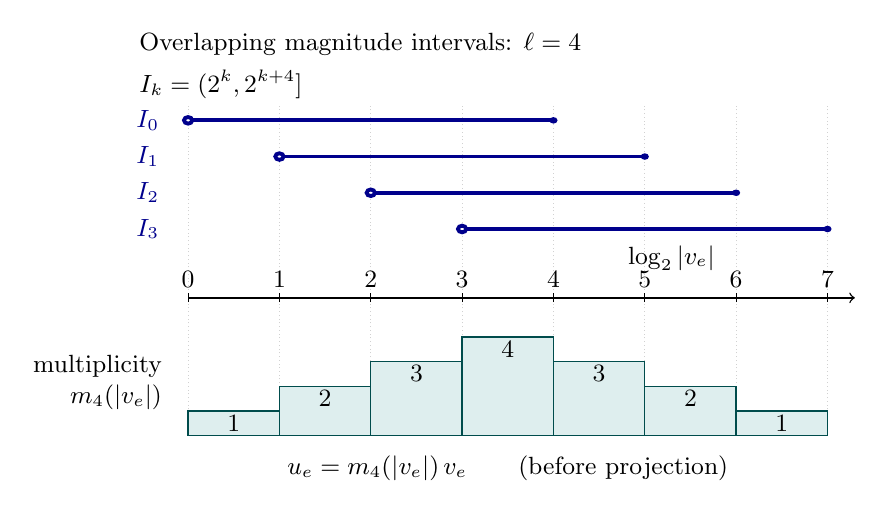
\begin{tikzpicture}[x=1.16cm,y=0.92cm,font=\small,
  every node/.style={inner sep=2pt},
  interval/.style={draw=blue!55!black,line width=1.4pt},
  guide/.style={draw=black!18,densely dotted,line width=0.35pt}]
  \node[anchor=west] at (-0.6,5.4)
    {Overlapping magnitude intervals: $\ell=4$};
  \node[anchor=west] at (-0.6,4.85)
    {$I_k=(2^k,2^{k+4}]$};
  \foreach \j in {0,...,7}{
    \draw[guide] (\j,0) -- (\j,4.55);
  }
  \foreach \k in {0,...,3}{
    \pgfmathsetmacro{\rightend}{\k+4}
    \pgfmathsetmacro{\rowheight}{4.35-0.5*\k}
    \node[anchor=east,text=blue!55!black] at (-0.25,\rowheight)
      {$I_{\k}$};
    \draw[interval] (\k,\rowheight) -- (\rightend,\rowheight);
    \draw[interval,fill=white] (\k,\rowheight) circle[radius=0.045];
    \fill[blue!55!black] (\rightend,\rowheight) circle[radius=0.045];
  }
  \draw[->,line width=0.5pt] (0,1.9) -- (7.3,1.9);
  \foreach \j in {0,...,7}{
    \draw (\j,1.84) -- (\j,1.96);
    \node[above] at (\j,1.96) {$\j$};
  }
  \node[anchor=west] at (4.75,2.45) {$\log_2|v_e|$};
  \foreach \j/\mult in {0/1,1/2,2/3,3/4,4/3,5/2,6/1}{
    \pgfmathsetmacro{\rightbin}{\j+1}
    \pgfmathsetmacro{\barheight}{0.34*\mult}
    \filldraw[fill=teal!13,draw=teal!60!black,line width=0.5pt]
      (\j,0) rectangle (\rightbin,\barheight);
    \node at ({\j+0.5},{\barheight-0.17}) {$\mult$};
  }
  \node[anchor=east,align=right] at (-0.22,0.73)
    {multiplicity\\$m_4(|v_e|)$};
  \node[anchor=north] at (3.5,-0.2)
    {$u_e=m_4(|v_e|)\,v_e\qquad\text{(before projection)}$};
\end{tikzpicture}

\caption{The overlapping truncations for $\ell=4$.
The intervals $I_k=(2^k,2^{k+4}]$, $0\le k<4$, give multiplicities
$1,2,3,4,3,2,1$ on $(2^j,2^{j+1}]$, $j=0,\ldots,6$, and zero
outside $(1,128]$. Thus $u_e=m_4(|v_e|)v_e$ before projection.
By the magnitude-density identity, a bin of multiplicity $m$
contributes $p\log 2\,m^p$ to $\int|u_e|^p\,d\nu$.}
\label{fig:truncation-ramp}
\end{figure}

The same identity gives
\[
 \int |v_e|^2\mathbf 1_{\{|v_e|>a\}}\,d\nu
   =\frac{p}{p-2}a^{2-p}.
\]
The triangle inequality in $L_2(\nu)$, applied to
\eqref{eq:above-ramp}, consequently yields
\[
 \left(\int |u_e|^2\,d\nu\right)^{1/2}
 \le \left(\frac{p}{p-2}\right)^{1/2}
       \sum_{k=0}^{\ell-1}2^{(1-p/2)k}
 \le C_p.
\]
Using the contraction of $P$ in $\ell_2(\sigma)$ and its row-sum bound,
we obtain
\begin{equation}
 \|Z\|_{L_2(\rho)}^2\le C_p,
 \qquad
 \sup_e\int |Z_e|^2\,d\nu\le C_pH^2,
 \qquad
 \sup_{e,r,t}|Z_e(r,t)|\le H2^{2\ell}.
\label{eq:above-basic-bounds}
\end{equation}
In particular, the coordinatewise quadratic estimate follows from
\[
 \left(\int|Z_e|^2\,d\nu\right)^{1/2}
 \le\sum_f|P_{ef}|\left(\int|u_f|^2\,d\nu\right)^{1/2}
 \le C_pH.
\]
For the supremum bound in~\eqref{eq:above-basic-bounds}, each summand
defining $u_e$ has magnitude at
most $2^{k+\ell}$, and their sum is less than $2^{2\ell}$.

\subsection{The projection error}

We claim that
\begin{equation}
 \|Z-u\|_{L_p(\rho)}^p
       \le C_p H^{p-2}(\ell+1).
 \label{eq:above-projection-error}
\end{equation}
For $0\le k<2\ell$, define the pointwise vector function
\[
 A_k=(P-I)v_{\le2^k}.
\]
Although $v_{\le2^k}$ need not belong to $L_2(\rho)$, the identity
$Pv=v$ holds pointwise and gives
$A_k=-(P-I)v_{>2^k}$. Thus $A_k$ does belong to $L_2(\rho)$, and
\begin{equation}
 \|A_k\|_\infty\le 2H2^k,
 \qquad
 \|A_k\|_{L_2(\rho)}\le C_p2^{(1-p/2)k}.
 \label{eq:above-cutoff-bounds}
\end{equation}
Here the second inequality uses the $\ell_2(\sigma)$ contraction of
$I-P$ and the preceding tail integral. Moreover,
\[
 Z-u=\sum_{k=\ell}^{2\ell-1}A_k-\sum_{k=0}^{\ell-1}A_k.
\]
Summing the two bounds in~\eqref{eq:above-cutoff-bounds} separately
shows that this signed sum has $L_2(\rho)$ norm at most $C_p$ and
supremum norm at most $CH2^{2\ell}$.

For a level $\tau\ge16H$, split the sum at
$2^k\le\tau/(16H)$. The sum of the supremum norms of these smaller
terms is at most $\tau/2$. By geometric decay, the remaining terms
have total $L_2(\rho)$ norm at most
$C_p(\tau/H)^{1-p/2}$. Chebyshev's inequality, together with the
global $L_2$ bound for smaller levels, gives
\[
 \rho\bigl(|Z-u|>\tau\bigr)\le
 \begin{cases}
 C_p\tau^{-2},&0<\tau<16H,\\
 C_pH^{p-2}\tau^{-p},&\tau\ge16H.
 \end{cases}
\]
This tail vanishes for $\tau>CH2^{2\ell}$. Integrating it against
$p\tau^{p-1}\,d\tau$ proves~\eqref{eq:above-projection-error}:
the smaller levels contribute $C_pH^{p-2}$, and the larger levels
contribute at most $C_pH^{p-2}(\ell+1)$.

Since $\|u\|_{L_p(\rho)}^p=b$, the pointwise power-difference
inequality and H\"older's inequality imply
\begin{align}
 \sum_e\sigma_e\left|\int|Z_e|^p\,d\nu-b\right|
 &\le p\|Z-u\|_{L_p(\rho)}
       \bigl(\|u\|_{L_p(\rho)}+
                    \|Z-u\|_{L_p(\rho)}\bigr)^{p-1}.
 \label{eq:above-energy-error}
\end{align}
By~\eqref{eq:above-energy} and~\eqref{eq:above-projection-error},
\begin{equation}
 \frac{\|Z-u\|_{L_p(\rho)}}{b^{1/p}}
       \le C_p\frac{H^\gamma}{\ell}.
 \label{eq:above-relative-error}
\end{equation}
Choose
\begin{equation}
 \ell=\left\lceil L H^\gamma\right\rceil,
 \label{eq:above-length}
\end{equation}
where $L\ge1$ depends only on $p,\eta$ and will be enlarged once
more below. First choose it large enough that
\eqref{eq:above-energy-error} is at most $\eta b/8$.

\subsection{Poisson sampling}

We need the leading coefficient in the next estimate to be arbitrarily
close to one, since the desired distortion $D$ may be arbitrarily
close to one.

\begin{lemma}[Nearly additive Poisson moments]\label{lem:poisson-moments}
Let $h$ be a bounded real function supported on a region of finite
$\nu$-measure, and let $S$ be its signed Poisson sum.
For $q>2$ and $\epsilon>0$,
\begin{equation}\label{eq:poisson-moments}
 \int|h|^q\,d\nu
 \le\E|S|^q
 \le(1+\epsilon)\int|h|^q\,d\nu
   +C_{q,\epsilon}\left(\int h^2\,d\nu\right)^{q/2}.
\end{equation}
\end{lemma}

A proof using independent symmetric sums is given in
Appendix~\ref{app:poisson}.

The function $Z$ vanishes outside
\[
 S=\{(r,t):\max_e|v_e(r,t)|>1\},
 \qquad \nu(S)\le |E|,
\]
because $u$ vanishes there. Hence we may take the signed Poisson sum
$W$ of $Z$ on this finite-measure region. Every summand is in $V$,
so $W\in V$ almost surely.

Write
$m_e=\int|Z_e|^p\,d\nu$ and $a_e=\int|Z_e|^2\,d\nu$.
Lemma~\ref{lem:poisson-moments} gives, for every $\epsilon>0$,
\[
 0\le \E|W_e|^p-m_e
      \le \epsilon m_e+C_{p,\epsilon}a_e^{p/2}.
\]
The two quadratic estimates in~\eqref{eq:above-basic-bounds} imply
\begin{equation}
 \sum_e\sigma_e a_e^{p/2}
 \le \left(\max_e a_e\right)^{p/2-1}\sum_e\sigma_e a_e
 \le C_pH^{p-2}.
 \label{eq:above-variance-error}
\end{equation}
Set $\epsilon=\eta/32$. The projection estimate gives
$\sum_e\sigma_e m_e\le(1+\eta/8)b$, so the averaged
$\epsilon m_e$ term is at most $\eta b/16$. Further,
\[
 \frac{H^{p-2}}{b}
 \le C_p\frac{H^{p-2}}{\ell^{p+1}}
 \le C_pL^{-(p+1)}H^{-\gamma}
 \le C_pL^{-(p+1)}.
\]
Enlarge $L$, still depending only on $p,\eta$, until the contribution
of~\eqref{eq:above-variance-error}, including its constant
$C_{p,\epsilon}$, is at most $\eta b/16$. We have proved
\begin{equation}
 \sum_e\sigma_e\left|\E|W_e|^p-b\right|
   \le \frac{\eta b}{8}+\frac{\eta b}{16}
                         +\frac{\eta b}{16}
   =\frac{\eta b}{4}.
 \label{eq:above-poisson-error}
\end{equation}

\subsection{A bounded random gradient}

Choose a constant $C_p'$ so that
\[
 J=C_p'H2^{2\ell}\ge1
\]
dominates both $\sup_{e,r,t}|Z_e(r,t)|$ and
$\sup_e a_e^{1/2}$. The exponential-moment formula for signed
Poisson sums gives
\[
 \E\exp(\pm W_e/J)
 =\exp\left(\int\bigl(\cosh(Z_e/J)-1\bigr)\,d\nu\right)
 \le e^{C_0},
\]
where $C_0$ is absolute: use
$\cosh s-1\le C_0s^2$ for $|s|\le1$ and $a_e\le J^2$.
Consequently, for $z\ge0$,
\begin{equation}
 \Prob(|W_e|>Jz)\le2e^{C_0-z},
 \qquad \E|W_e|^{2p}\le C_pJ^{2p}.
 \label{eq:above-poisson-tail}
\end{equation}
Set
\[
 K=8J\log(2n),\qquad
 \mathcal B=\{\max_e|W_e|>K\},\qquad
 F=W\mathbf 1_{\mathcal B^c}.
\]
Discarding the entire vector on a bad event preserves membership in
$V$, so $F\in V$ and $\|F\|_\infty\le K$. By the union bound and
\eqref{eq:above-poisson-tail},
\[
 \Prob(\mathcal B)
 \le2|E|e^{C_0}(2n)^{-8}\le Cn^{-6}.
\]
For every edge, Cauchy--Schwarz therefore gives
\begin{equation}
 0\le\E|W_e|^p-\E|F_e|^p
   \le (\E|W_e|^{2p})^{1/2}\Prob(\mathcal B)^{1/2}
   \le C_pJ^pn^{-3}.
 \label{eq:above-truncation-error}
\end{equation}
By~\eqref{eq:above-length},
\[
 \log J=O_{p,\eta}(H^\gamma)=o(\log n).
\]
Thus the last bound in~\eqref{eq:above-truncation-error} tends to
zero uniformly over the input points and $\lambda$. Since $b\ge1$,
it is at most $\eta b/4$ for all sufficiently large $n$, with the
threshold depending only on $p,\eta$. Combining this with
\eqref{eq:above-poisson-error} and $\lambda\le2\sigma$ yields
\[
 \sum_e\lambda_e\left|\E|F_e|^p-b\right|
 \le2\sum_e\sigma_e\left|\E|F_e|^p-b\right|
 \le\eta b.
\]
The parameters $b\ge1$ and $K\ge1$ are independent of $\lambda$
and of the input points, as required by Lemma~\ref{lem:weighted}.
Finally,
\[
 \log K=O_{p,\eta}(H^\gamma)
         =O_{p,\eta}\bigl((\log n)^{1-2/p}\bigr).
\]
These are the parameters required by Lemma~\ref{lem:weighted} in this range.

\section{Dimension bounds and exact embeddings}

Table~\ref{tab:moment-contract} summarizes the common parameters supplied
by the two constructions. The target moment and magnitude bound are fixed
before the test probability $\lambda$ varies; the projection and the joint
law of the random gradient may depend on that probability.

\begin{table}[ht]
\centering
\renewcommand{\arraystretch}{1.4}
\begin{tabular}{ccl}
Range & Common moment $b$ & Magnitude bound $K$ \\
\hline
$1<p<2$ & $\E\min\{|Y_e|,T/H\}^p$ & $HT$ \\
$p>2$ & $p\log2\bigl(\ell^p+2\sum_{1\le j<\ell}j^p\bigr)$
       & $8J\log(2n)$
\end{tabular}
\caption{The weighted-moment contract for sufficiently large $n$.
Here $T=\exp(A_{p,\eta}H^{2-p})$, $\ell=\lceil LH^{1-2/p}\rceil$
in their respective ranges, and $J=C'_pH2^{2\ell}$.
All these choices are independent of the input points and pair weights.}
\label{tab:moment-contract}
\end{table}

\subsection{Completion of the upper bound}

In Sections~\ref{sec:below} and~\ref{sec:above}, the constructed
parameters satisfy $b,K\ge1$, the weighted moment condition
\eqref{eq:weighted-target}, and
\[
 \log K\le C_{p,\eta}(\log n)^{\gamma(p)}
\]
for all sufficiently large $n$, with a threshold depending only on
$p,\eta$. Lemma~\ref{lem:weighted} and~\eqref{eq:eta-choice} give
an embedding of distortion at most $D$. Since $b\ge1$, its dimension
satisfies
\[
 \log d\le C_{p,\eta}+2p\log K+\log\log(2n)
 \le C_{p,D}(\log n)^{\gamma(p)}.
\]
This proves the upper bound in~\eqref{eq:main-bounds} for sufficiently
large $n$. For the remaining finitely many values of $n$, enlarge
$C_{p,D}$ and use Lemma~\ref{lem:exact-upper}.

\subsection{The packing bound}

The coordinate unit vectors in $\ell_p^n$ form an equilateral set.
After translating and scaling any distortion-$D$ image in $\ell_p^d$,
its points are $1$-separated and lie in the ball of radius $D$ about
the first point. Their open balls of radius $1/2$ are disjoint and
lie in the ball of radius $D+1/2$ about that point. Comparing
$d$-dimensional Lebesgue volumes gives
\[
 n(1/2)^d\le(D+1/2)^d,
 \qquad\text{hence}\qquad n\le(1+2D)^d.
\]
This proves the lower bound in~\eqref{eq:main-bounds}.

\subsection{A quadratic obstruction to exact embeddings}

For real $a,b$, define
\[
 \Delta_p(a,b)=|a+b|^p+|a-b|^p-2|a|^p-2|b|^p.
\]
If $ab=0$, this is zero. If $ab\ne0$, it has strictly the sign of
$p-2$. To verify this, apply convexity for $p>2$, or concavity for
$p<2$, to the two numbers $(a+b)^2$ and $(a-b)^2$ raised to the power
$p/2$. Their average is $a^2+b^2$. Next use the strict inequality
\[
 (a^2+b^2)^{p/2}
 \begin{cases}
  >|a|^p+|b|^p,&p>2,\\
  <|a|^p+|b|^p,&p<2.
 \end{cases}
\]
Thus, for $u,v\in\ell_p^d$ and $p\ne2$,
\begin{equation}\label{eq:disjointness}
 \|u+v\|_p^p+\|u-v\|_p^p
 =2\|u\|_p^p+2\|v\|_p^p
 \quad\Longleftrightarrow\quad
 \operatorname{supp}(u)\cap\operatorname{supp}(v)=\varnothing.
\end{equation}
Indeed, the difference of the two sides is
$\sum_{a=1}^d\Delta_p(u_a,v_a)$, whose nonzero summands all have the
same sign.

Fix $k\ge2$. Index the coordinates of $\ell_p^{k^2}$ by
$\{1,\ldots,k\}^2$. Let $r_i$ be the indicator of row $i$, and $c_j$
the indicator of column $j$. Consider the $4k+1$ distinct points
\[
 \mathcal X_k=\{0\}\cup\{r_i,-r_i:1\le i\le k\}
                    \cup\{c_j,-c_j:1\le j\le k\}.
\]
Suppose that $\mathcal X_k$ embeds with distortion one into
$\ell_p^d$. Translate and rescale to obtain an isometry $f$ with
$f(0)=0$. Strict convexity of $\ell_p^d$ implies
\begin{equation}\label{eq:antipodes}
 f(-x)=-f(x)\qquad(x\in\mathcal X_k).
\end{equation}
In fact, $\|f(x)-f(-x)\|_p=2\|x\|_p$ and both $\|f(x)\|_p$ and
$\|f(-x)\|_p$ equal $\|x\|_p$, so equality in the triangle inequality
forces the two vectors $f(x)$ and $-f(-x)$ to coincide.

By~\eqref{eq:antipodes}, the expression in~\eqref{eq:disjointness}
is determined by distances among the given points and is preserved
by $f$. Distinct rows have disjoint supports, so the supports of
$f(r_1),\ldots,f(r_k)$ are pairwise disjoint. The same holds for
$f(c_1),\ldots,f(c_k)$. In contrast, each row and column intersect
in exactly one coordinate. Their defect is
\[
 \|r_i+c_j\|_p^p+\|r_i-c_j\|_p^p
 -2\|r_i\|_p^p-2\|c_j\|_p^p=2^p-4\ne0.
\]
Consequently $\operatorname{supp}(f(r_i))$ meets
$\operatorname{supp}(f(c_j))$ for every $(i,j)$. A single coordinate
can belong to at most one row support and at most one column support,
so it can account for at most one of these $k^2$ intersections.
It follows that $d\ge k^2$.

For $n\ge9$, take $k=\lfloor(n-1)/4\rfloor$ and add distinct points
if necessary to obtain an $n$-point set. Any exact embedding of that
set restricts to one of $\mathcal X_k$, proving the lower bound
in~\eqref{eq:exact-bounds}. The upper bound is
Lemma~\ref{lem:exact-upper}. Finally, $0<\gamma(p)<1$, so the
logarithmic limits in Theorem~\ref{thm:main} follow from the stated
bounds.


\appendix
\section{Electrical-flow localization}\label{app:localization}

The following proof follows the heat-kernel and entropy argument of
Gurel-Gurevich, Nachmias, and Sachdeva~\cite[Sections~2--4]{GGNS},
in the symmetric projection notation used here.

\begin{proof}[Proof of Lemma~\ref{lem:localization}]
Fix a strictly positive edge vector $w$, and define a vertex probability
measure and its diagonal matrix by
\[
  \mu_i=\frac{\sum_{e\ni i}w_e^2}{2\|w\|_2^2},
  \qquad M=\operatorname{diag}(\mu_i).
\]
Connectivity implies $\mu_i>0$. Put
\[
  L=B^TCB,\qquad S=M^{-1/2}LM^{-1/2},\qquad
  K_t=M^{-1/2}e^{-tS}M^{-1/2}.
\]
Writing $A=C^{1/2}BM^{-1/2}$, we have $S=A^TA$ and
$\operatorname{im}A=\operatorname{im}(C^{1/2}B)$. Spectral decomposition
therefore gives the convergent matrix integral
\begin{equation}\label{eq:projection-heat-integral}
 Q=\int_0^\infty C^{1/2}BK_tB^TC^{1/2}\,dt.
\end{equation}
Indeed, the integrand is $Ae^{-tA^TA}A^T$, whose integral is the
orthogonal projection onto $\operatorname{im}A$.

For a vertex $v$, set $h_s=K_s\mathbf e_v$, where $\mathbf e_v$ is the
$v$-th coordinate vector. The identity
\[
 K_s=e^{-sM^{-1}L}M^{-1}
\]
shows that $h_s$ has strictly positive coordinates for $s>0$:
the matrix $-M^{-1}L$ has nonnegative off-diagonal entries, and after
adding a sufficiently large multiple of the identity, its exponential
is strictly positive by connectivity and the power series for the
exponential. Moreover,
\[
 \mu^Th_s=1,\qquad
 h_s\longrightarrow\mathbf 1\quad(s\to\infty),\qquad
 h_0=\mu_v^{-1}\mathbf e_v.
\]
Mass conservation follows from $\mathbf 1^TL=0$; the limit follows
from the spectral decomposition of $S$, whose kernel is spanned by
$M^{1/2}\mathbf 1$, a unit vector.

For a positive vertex vector $h$, define
\[
 \mathcal I(h)=\sum_{e=ij}c_e(h(i)-h(j))
                    (\log h(i)-\log h(j)).
\]
Using $\partial_sh_s=-M^{-1}Lh_s$ and mass conservation, we obtain
\[
 \frac{d}{ds}\sum_i\mu_i h_s(i)\log h_s(i)
   =-h_s^TL\log h_s=-\mathcal I(h_s).
\]
Integrating first over a compact subinterval of $(0,\infty)$ and then
taking the endpoints to $0$ and $\infty$ gives
\begin{equation}\label{eq:heat-entropy}
 \int_0^\infty\mathcal I(h_s)\,ds=\log(1/\mu_v).
\end{equation}
Here $0\log0=0$, so continuity gives the entropy at time $0$ as
$\log(1/\mu_v)$, whereas its limit at infinity is $0$.

For $a,b>0$, with the continuous interpretation when $a=b$,
\[
 \frac{a-b}{\log a-\log b}
   =\int_0^1a^ub^{1-u}\,du\le\frac{a+b}{2}.
\]
Cauchy--Schwarz and $\mu^Th_s=1$ consequently yield
\begin{align}
 \bigl(w^TC^{1/2}|Bh_s|\bigr)^2
 &\le \mathcal I(h_s)
          \sum_{e=ij}w_e^2\frac{h_s(i)+h_s(j)}2 \notag\\
 &=\mathcal I(h_s)\|w\|_2^2.
 \label{eq:heat-cauchy-schwarz}
\end{align}
Since $K_{2s}=K_sMK_s$, substituting $t=2s$ in
\eqref{eq:projection-heat-integral}, expanding $K_sMK_s$ into column
outer products, and applying the triangle inequality gives
\begin{align*}
 w^T|Q|w
 &\le 2\sum_v\mu_v\int_0^\infty
       \bigl(w^TC^{1/2}|BK_s\mathbf e_v|\bigr)^2\,ds\\
 &\le 2\|w\|_2^2\sum_v\mu_v\log(1/\mu_v)
 \le 2\|w\|_2^2\log n,
\end{align*}
by \eqref{eq:heat-entropy} and \eqref{eq:heat-cauchy-schwarz}.
Continuity extends this bound to nonnegative $w$. Finally, $|Q|$ is
symmetric and entrywise nonnegative, so for every real vector $x$,
\[
 \bigl|x^T|Q|x\bigr|
 \le |x|^T|Q||x|\le 2\log n\,\|x\|_2^2.
\]
This proves \eqref{eq:localization}.
\end{proof}

\section{The Poisson moment inequality}\label{app:poisson}

\begin{proof}[Proof of Lemma~\ref{lem:poisson-moments}]
We prove the moment bounds first for a sum of independent symmetric
real random variables $X_1,\ldots,X_N$ with finite $q$th moments.
For real $a,b$,
\begin{equation}\label{eq:scalar-lower}
 \frac{|a+b|^q+|a-b|^q}{2}\ge|a|^q+|b|^q.
\end{equation}
Indeed, convexity of $u\mapsto u^{q/2}$ first bounds the left side
below by $(a^2+b^2)^{q/2}$, which is at least $|a|^q+|b|^q$.
Iterating~\eqref{eq:scalar-lower} proves the lower moment bound.

For every $\epsilon'>0$ there is $C_{q,\epsilon'}$ such that
\begin{equation}\label{eq:scalar-upper}
 \frac{|a+b|^q+|a-b|^q}{2}
 \le |a|^q+(1+\epsilon')|b|^q
    +C_{q,\epsilon'}|a|^{q-2}|b|^2.
\end{equation}
To see this, the case $a=0$ is immediate. Otherwise divide by $|a|^q$
and put $u=b/a$. Near $u=0$, Taylor's theorem bounds the left side
minus $1$ by $C_qu^2$. For sufficiently large $|u|$, the left side
divided by $|u|^q$ is at most $1+\epsilon'$. On the remaining compact
set, enlarge the coefficient of $u^2$.

Let $S_j=X_1+\cdots+X_j$ and $M_q=\E|S_N|^q$. Each $S_j$ is the
conditional expectation of $S_N$ given $X_1,\ldots,X_j$, so
$\E|S_j|^q\le M_q$. Independence, symmetry, and
\eqref{eq:scalar-upper} give
\[
 M_q\le(1+\epsilon')\sum_{j=1}^N\E|X_j|^q
  +C_{q,\epsilon'}M_q^{1-2/q}\sum_{j=1}^N\E|X_j|^2.
\]
Young's inequality bounds the last term by
$\theta M_q+C_{q,\epsilon',\theta}(\sum_j\E|X_j|^2)^{q/2}$.
Choose $\epsilon',\theta>0$ so that
$(1+\epsilon')/(1-\theta)\le1+\epsilon$, and absorb $\theta M_q$.
This proves the asserted independent-sum bounds.

To pass to a Poisson sum on a region of mass $M>0$, take $N>M$
independent trials, each equal to an independent signed sample with
probability $M/N$ and zero otherwise. The sums of their $q$th and
second moments are exactly $\int|h|^q\,d\nu$ and $\int h^2\,d\nu$.
Their activation count converges in law to a Poisson variable of
mean $M$. Conditional on that count, their nonzero samples have the
desired law. If $B_N$ is the activation count, then
\[
 \E e^{B_N}=\left(1+\frac{M(e-1)}N\right)^N\le e^{M(e-1)}.
\]
Since $h$ is bounded, these exponential bounds give uniform
integrability of the $q$th powers of the sums. Weak convergence followed
by truncation therefore gives convergence of their $q$th moments;
see also~\cite[Sections~3.2 and~4.6]{Durrett2019} for these standard
convergence principles. The independent-sum bounds therefore imply
\eqref{eq:poisson-moments}. The case $M=0$ is immediate.
\end{proof}


\begin{thebibliography}{99}
\addcontentsline{toc}{section}{References}
\bibitem{Ball1990}
Keith Ball.
\newblock Isometric embedding in $l_p$-spaces.
\newblock \emph{European Journal of Combinatorics}, 11(4):305--311, 1990.
\newblock \href{https://doi.org/10.1016/S0195-6698(13)80131-X}
{doi:10.1016/S0195-6698(13)80131-X}.

\bibitem{Bourgain1985}
Jean Bourgain.
\newblock On Lipschitz embedding of finite metric spaces in Hilbert space.
\newblock \emph{Israel Journal of Mathematics}, 52(1--2):46--52, 1985.
\newblock \href{https://doi.org/10.1007/BF02776078}{doi:10.1007/BF02776078}.

\bibitem{BourgainLindenstraussMilman1989}
Jean Bourgain, Joram Lindenstrauss, and Vitali Milman.
\newblock Approximation of zonoids by zonotopes.
\newblock \emph{Acta Mathematica}, 162:73--141, 1989.
\newblock \href{https://doi.org/10.1007/BF02392835}{doi:10.1007/BF02392835}.

\bibitem{BrinkmanCharikar2005}
Bo Brinkman and Moses Charikar.
\newblock On the impossibility of dimension reduction in $\ell_1$.
\newblock \emph{Journal of the ACM}, 52(5):766--788, 2005.
\newblock \href{https://doi.org/10.1145/1089023.1089026}
{doi:10.1145/1089023.1089026}.

\bibitem{Durrett2019}
Rick Durrett.
\newblock \emph{Probability: Theory and Examples}.
\newblock Author-posted manuscript, Version 5, January 11, 2019.
\newblock \url{https://sites.math.duke.edu/~rtd/PTE/PTE5_011119.pdf}.

\bibitem{Eskenazis2024}
Alexandros Eskenazis.
\newblock $\varepsilon$-isometric dimension reduction for incompressible
subsets of $\ell_p$.
\newblock \emph{Discrete \& Computational Geometry}, 71:160--176, 2024.
\newblock \href{https://doi.org/10.1007/s00454-023-00587-w}
{doi:10.1007/s00454-023-00587-w}.

\bibitem{GGNS}
Ori Gurel-Gurevich, Asaf Nachmias, and Sushant Sachdeva.
\newblock \emph{A Tight Bound on Localization of Electrical Flows}.
\newblock arXiv:2605.24130v1, 2026.
\newblock \href{https://arxiv.org/abs/2605.24130v1}{arxiv.org/abs/2605.24130v1}.

\bibitem{Hatcher2002}
Allen Hatcher.
\newblock \emph{Algebraic Topology}.
\newblock Cambridge University Press, Cambridge, 2002.
\newblock \url{https://pi.math.cornell.edu/~hatcher/AT/AT.pdf}.

\bibitem{Hoeffding1963}
Wassily Hoeffding.
\newblock Probability inequalities for sums of bounded random variables.
\newblock \emph{Journal of the American Statistical Association},
58(301):13--30, 1963.
\newblock \href{https://doi.org/10.1080/01621459.1963.10500830}
{doi:10.1080/01621459.1963.10500830}.

\bibitem{Indyk06}
Piotr Indyk.
\newblock Stable distributions, pseudorandom generators, embeddings,
and data stream computation.
\newblock \emph{Journal of the ACM}, 53(3):307--323, 2006.

\bibitem{JohnsonLindenstrauss1984}
William B. Johnson and Joram Lindenstrauss.
\newblock Extensions of Lipschitz mappings into a Hilbert space.
\newblock In \emph{Conference in Modern Analysis and Probability},
Contemporary Mathematics, volume 26, pages 189--206.
American Mathematical Society, Providence, RI, 1984.
\newblock \href{https://doi.org/10.1090/conm/026/737400}
{doi:10.1090/conm/026/737400}.

\bibitem{Lamperti1958}
John Lamperti.
\newblock On the isometries of certain function-spaces.
\newblock \emph{Pacific Journal of Mathematics}, 8(3):459--466, 1958.
\newblock \href{https://doi.org/10.2140/pjm.1958.8.459}
{doi:10.2140/pjm.1958.8.459}.

\bibitem{LeeMendelNaor2005}
James R. Lee, Manor Mendel, and Assaf Naor.
\newblock Metric structures in $L_1$: dimension, snowflakes, and average
distortion.
\newblock \emph{European Journal of Combinatorics}, 26(8):1180--1190, 2005.
\newblock \href{https://doi.org/10.1016/j.ejc.2004.07.002}
{doi:10.1016/j.ejc.2004.07.002}.

\bibitem{LeeNaor2004}
James R. Lee and Assaf Naor.
\newblock Embedding the diamond graph in $L_p$ and dimension reduction
in $L_1$.
\newblock \emph{Geometric and Functional Analysis}, 14(4):745--747, 2004.
\newblock \href{https://doi.org/10.1007/s00039-004-0473-8}
{doi:10.1007/s00039-004-0473-8}.

\bibitem{Naor2018}
Assaf Naor.
\newblock Metric dimension reduction: a snapshot of the Ribe program.
\newblock In \emph{Proceedings of the International Congress of
Mathematicians---Rio de Janeiro 2018}, volume I, pages 759--837.
World Scientific, 2018.
\newblock \href{https://arxiv.org/abs/1809.02376v1}{arXiv:1809.02376v1}.

\bibitem{NaorRen2026Threshold}
Assaf Naor and Kevin Ren.
\newblock \emph{A threshold phenomenon for embeddings of Euclidean
snowflakes and impossibility of dimension reduction}.
\newblock arXiv:2609.01079v1, 2026.
\newblock \href{https://arxiv.org/abs/2609.01079v1}{arxiv.org/abs/2609.01079v1}.

\bibitem{OpenAI2026DoublingHilbert}
OpenAI.
\newblock \emph{A doubling Hilbert subset with no finite-dimensional
bi-Lipschitz embedding}.
\newblock OpenAI Math Release preprint
\href{https://github.com/openai/math/blob/main/preprints/A-doubling-Hilbert-subset-with-no-finite-dimensional-bi-Lipschitz-embedding-September-25-2026/main.pdf}{OAI:A-doubling-Hilbert-subset-with-no-finite-dimensional-bi-Lipschitz-embedding-September-25-2026},
2026.

\bibitem{Pinelis15}
Iosif Pinelis.
\newblock Exact Rosenthal-type bounds.
\newblock \emph{The Annals of Probability}, 43(5):2511--2544, 2015.
\newblock \href{https://doi.org/10.1214/14-AOP942}{doi:10.1214/14-AOP942}.

\bibitem{Pisier1981}
Gilles Pisier.
\newblock Remarques sur un r\'esultat non publi\'e de B. Maurey.
\newblock \emph{S\'eminaire d'analyse fonctionnelle}, 1980--1981,
Expos\'e no.~5, pages 1--12. \'Ecole Polytechnique, Palaiseau, 1981.
\newblock \url{https://numdam.org/item/SAF_1980-1981____A5_0/}.

\bibitem{Rockafellar1970}
R. Tyrrell Rockafellar.
\newblock \emph{Convex Analysis}.
\newblock Princeton Mathematical Series, volume 28.
Princeton University Press, Princeton, NJ, 1970; second printing, 1972.

\bibitem{Rosenthal70}
Haskell P. Rosenthal.
\newblock On the subspaces of $L^p$ $(p>2)$ spanned by sequences of
independent random variables.
\newblock \emph{Israel Journal of Mathematics}, 8:273--303, 1970.
\newblock \href{https://doi.org/10.1007/BF02771562}{doi:10.1007/BF02771562}.

\bibitem{Schechtman1987}
Gideon Schechtman.
\newblock More on embedding subspaces of $L_p$ in $l_r^n$.
\newblock \emph{Compositio Mathematica}, 61(2):159--169, 1987.
\newblock \url{https://numdam.org/item/CM_1987__61_2_159_0/}.

\bibitem{Schechtman2011}
Gideon Schechtman.
\newblock \emph{Dimension reduction in $L_p$, $0<p<2$}.
\newblock arXiv:1110.2148v1, 2011.
\newblock \href{https://arxiv.org/abs/1110.2148v1}{arxiv.org/abs/1110.2148v1}.

\bibitem{SRS18}
Aaron Schild, Satish Rao, and Nikhil Srivastava.
\newblock Localization of electrical flows.
\newblock In \emph{Proceedings of the Twenty-Ninth Annual ACM-SIAM
Symposium on Discrete Algorithms}, pages 1577--1584, 2018.
\newblock \href{https://doi.org/10.1137/1.9781611975031.103}
{doi:10.1137/1.9781611975031.103}.
\newblock Preprint version: \href{https://arxiv.org/abs/1708.01632v1}
{arXiv:1708.01632v1}.

\bibitem{Talagrand1995}
Michel Talagrand.
\newblock Embedding subspaces of $L_p$ in $\ell_p^N$.
\newblock In \emph{Geometric Aspects of Functional Analysis},
Operator Theory: Advances and Applications, volume 77, pages 311--326.
Birkh\"auser, Basel, 1995.
\newblock \href{https://doi.org/10.1007/978-3-0348-9090-8_26}
{doi:10.1007/978-3-0348-9090-8\_26}.
\end{thebibliography}
\end{document}
